\documentclass[11pt,a4paper]{article}

\usepackage[utf8]{inputenc}
\usepackage[T1]{fontenc}
\usepackage[french]{babel}
\usepackage[a4paper,margin=2.4cm]{geometry}
\usepackage{graphicx}
\usepackage{booktabs}
\usepackage{array}
\usepackage{xcolor}
\usepackage{caption}
\usepackage{enumitem}
\usepackage{fancyhdr}
\usepackage{titlesec}
\usepackage[hidelinks]{hyperref}

\graphicspath{{figures/}}
\definecolor{nblue}{HTML}{1D3A6B}
\definecolor{acc}{HTML}{2563EB}
\definecolor{boxbg}{HTML}{EFF4FB}

\titleformat{\section}{\Large\bfseries\color{nblue}}{\thesection}{0.6em}{}
\titleformat{\subsection}{\large\bfseries\color{acc}}{\thesubsection}{0.6em}{}
\setlength{\parskip}{0.45em}

\pagestyle{fancy}\fancyhf{}
\lhead{\small\color{nblue}Analyse NLP des rapports d'incidents ASRS}
\rhead{\small\thepage}
\renewcommand{\headrulewidth}{0.4pt}
\captionsetup{font=small,labelfont={bf,color=nblue}}

% Encadré « pourquoi ce choix »
\newcommand{\pourquoi}[1]{%
  \par\smallskip\noindent\colorbox{boxbg}{\parbox{\dimexpr\linewidth-2\fboxsep}{%
  \small\textbf{\color{acc}Pourquoi ce choix pour le projet ?} #1}}\par\smallskip}

% Citation de récit réel
\newenvironment{narr}{%
  \begin{list}{}{\setlength{\leftmargin}{1.2em}\setlength{\rightmargin}{1.2em}}\item[]%
  \small\itshape\color{nblue}\guillemotleft~}{~\guillemotright\end{list}}

\begin{document}

% ---------- TITLE ----------
\begin{titlepage}
\centering
\vspace*{1.3cm}
{\small\color{acc}\textbf{AÉRONAUTIQUE \;|\; PROJET A3 \;|\; NLP · CLASSIFICATION · CLUSTERING}}\\[1.0cm]
{\color{nblue}\Huge\bfseries Analyse NLP des rapports\\[0.3cm] d'incidents de sécurité aérienne\par}
\vspace{0.45cm}
{\large Extraction des causes récurrentes, classification des anomalies\\ et détection de signaux faibles sur la base \textbf{NASA ASRS}\par}
\vspace{0.30cm}
{\itshape Rapport technique — version pédagogique\par}
\vspace{0.5cm}
{\large\bfseries Mehdi Tidjani \quad\textbullet\quad [Étudiant 2] \quad\textbullet\quad [Étudiant 3]\par}
\vspace{0.8cm}
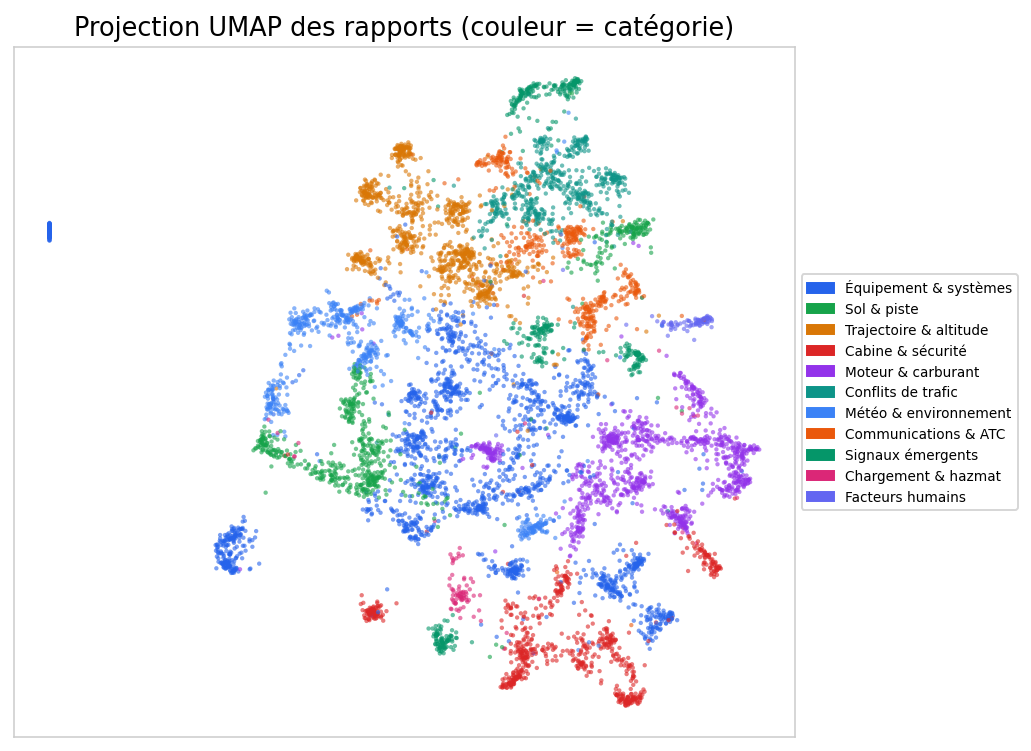
\includegraphics[width=0.90\textwidth]{scatter.png}\\[0.2cm]
{\small\itshape Projection sémantique des 125\,763 rapports, colorée par catégorie d'incident}
\vfill
\begin{tabular}{rl}
\textbf{Jeu de données} & NASA ASRS — 125\,763 rapports (2002–2025)\\
\textbf{Cadre} & Projet A3 — équipe de 3 étudiants \;|\; 3–4 semaines\\
\textbf{Livrables} & Pipeline NLP · Dashboards (Streamlit \& React) · Rapport\\
\textbf{Dépôt} & \url{https://github.com/devMehdi485/asrs-ml}\\
\end{tabular}
\vspace{0.8cm}
\end{titlepage}

% ---------- ABSTRACT ----------
\thispagestyle{empty}
\vspace*{2cm}
\begin{abstract}
\noindent Le présent rapport documente un projet de \textbf{traitement automatique du
langage naturel} appliqué à 125\,763 rapports d'incidents de la base \emph{Aviation Safety
Reporting System} (ASRS) de la NASA. Son objectif est de transformer une grande quantité de
récits écrits en texte libre en informations claires et exploitables pour la sécurité
aérienne. La démarche enchaîne cinq grandes étapes : nettoyer les textes, les convertir en
nombres, les regrouper par thème, identifier les sujets dominants, et enfin prédire le type
d'incident. Le document est volontairement rédigé de façon pédagogique : chaque terme
technique est expliqué lors de sa première apparition, et chaque choix de méthode est
justifié. Les résultats — 81 thèmes regroupés en 11 grandes familles, une classification
atteignant un score F1 pondéré de 0,615, et la détection de risques émergents (drones,
brouillage GPS, batteries au lithium) — sont systématiquement reliés aux enjeux
opérationnels de la sécurité aérienne.

\bigskip
\noindent\textbf{Mots-clés :} traitement du langage, sécurité aérienne, ASRS,
regroupement de textes, classification, détection d'anomalies.
\end{abstract}
\newpage

\tableofcontents
\newpage

% ---------- 1 ----------
\section{Contexte et problématique}

La base \emph{Aviation Safety Reporting System} (ASRS) rassemble des centaines de milliers
de rapports d'incidents, soumis volontairement par les pilotes, contrôleurs et techniciens
du transport aérien. Chaque rapport contient un \textbf{récit en texte libre} : une
personne y raconte, avec ses propres mots, un événement qui a compromis ou failli
compromettre la sécurité d'un vol.

Cette richesse est aussi la principale difficulté. L'information utile n'est pas rangée dans
des cases : elle est noyée dans des paragraphes rédigés à la main, tous différents. Or un
volume de 125\,000 récits ne peut pas être lu, mémorisé et recoupé par un être humain.

La problématique du projet est donc la suivante : \textbf{comment exploiter
automatiquement ces récits pour en extraire les causes récurrentes d'incidents, en
classer les types, et repérer les signaux faibles susceptibles d'annoncer de futurs
accidents ?} Pour répondre à cette question, le projet s'appuie sur le \textbf{NLP (Natural
Language Processing, ou traitement automatique du langage naturel)} : il s'agit de
l'ensemble des techniques permettant à un ordinateur d'analyser et de « comprendre » du
texte écrit en langage humain. C'est cette discipline qui va permettre de structurer,
regrouper et hiérarchiser automatiquement le contenu des rapports.

% ---------- 2 ----------
\section{Objectifs}

\begin{enumerate}[leftmargin=1.5em]
  \item \textbf{Extraction des causes récurrentes} : faire émerger automatiquement, sans
  liste prédéfinie, les grands thèmes d'incidents présents dans les rapports.
  \item \textbf{Classification des anomalies} : prédire la catégorie d'anomalie d'un rapport
  à partir de son texte.
  \item \textbf{Détection de signaux faibles} : repérer les rapports atypiques décrivant des
  phénomènes rares et potentiellement précurseurs.
\end{enumerate}

% ---------- 3 ----------
\section{Méthodologie : une chaîne de traitement en cinq temps}

La méthode suit un enchaînement logique, où chaque étape prépare la suivante : on commence
par \emph{nettoyer} le texte, puis on le \emph{transforme en nombres}, ce qui permet ensuite
de \emph{regrouper} les rapports, d'en \emph{extraire les sujets}, et enfin de \emph{prédire}
le type d'incident. Cette section décrit chaque étape et justifie le choix retenu.

\subsection{Étape 1 — Préparer les données et nettoyer les textes}
L'étude porte sur 125\,763 rapports (2002–2025). Les récits sont disponibles pour tous les
rapports, et les informations clés sont presque toujours renseignées (type d'anomalie
99,7\,\%, phase de vol 95,9\,\%, type d'aéronef 98,9\,\%, date 100\,\%). Les données
proviennent de l'outil officiel de la NASA ; un jeu équivalent est aussi diffusé sur
\textbf{Kaggle} (une plateforme publique de jeux de données et de notebooks), utilisé ici
comme source complémentaire pour la reproductibilité et la comparaison avec d'autres
travaux.

Les textes subissent ensuite un \textbf{nettoyage} : on enlève les marqueurs
d'anonymisation, on met tout en minuscules, on découpe les phrases en mots, on retire les
mots très courants sans valeur informative, et on ramène chaque mot à sa forme de base.
\pourquoi{Le nettoyage sert simplement à réduire le « bruit » — c'est-à-dire tout ce qui
parasite l'analyse — pour que les méthodes suivantes se concentrent sur les mots réellement
porteurs de sens.}

\subsection{Étape 2 — Transformer le texte en nombres (vectorisation)}
Un ordinateur ne manipule pas des mots mais des nombres. Il faut donc convertir chaque
rapport en une suite de nombres : c'est la \textbf{vectorisation}. Trois représentations
complémentaires sont utilisées.

\textbf{TF-IDF (Term Frequency – Inverse Document Frequency, soit « fréquence du terme –
fréquence inverse de document »)} est une méthode qui attribue à chaque mot un poids
d'autant plus élevé qu'il est fréquent dans un rapport mais rare dans l'ensemble du corpus.
Un mot banal partout obtient un poids faible ; un mot spécifique obtient un poids fort.
\pourquoi{TF-IDF est simple, rapide et surtout \emph{interprétable} : on peut lire
directement quels mots caractérisent un thème. Elle sert de base à la classification et à la
description des groupes.}

\textbf{Word2Vec} est une méthode qui apprend, pour chaque mot, un vecteur numérique tel que
les mots de sens proche se retrouvent proches dans l'espace. Entraînée sur le corpus, elle
« apprend » le vocabulaire du domaine aéronautique.
\pourquoi{Word2Vec permet de vérifier que les données et le nettoyage sont cohérents : si le
modèle place correctement les mots proches, c'est que le signal sémantique est bien présent.}

Enfin, chaque rapport entier est transformé en un \textbf{vecteur numérique appelé
\emph{embedding}}, qui représente le \emph{sens global} du texte (et pas seulement des mots
isolés). Deux récits décrivant la même situation avec des mots différents auront des
embeddings proches. Ces embeddings sont produits par un \textbf{Sentence Transformer}
(modèle de phrases, ici \texttt{all-MiniLM-L6-v2}) : un réseau de neurones pré-entraîné qui
encode une phrase complète en un seul vecteur.
\pourquoi{Les embeddings de phrases captent le sens d'un récit même quand le vocabulaire
varie d'un pilote à l'autre ; ils donnent donc des regroupements bien plus cohérents que les
seuls mots.}

\subsection{Étape 3 — Regrouper les rapports par thème (clustering)}
Le \textbf{clustering} (ou regroupement automatique) consiste à rassembler les rapports qui
se ressemblent, sans étiquette préalable. Avant de regrouper, les embeddings (qui comportent
des centaines de dimensions) sont compressés grâce à \textbf{UMAP (Uniform Manifold
Approximation and Projection)}, une technique de \emph{réduction de dimension} : elle projette
les vecteurs dans un espace beaucoup plus petit tout en préservant les proximités entre
points.
\pourquoi{UMAP réduit le bruit, accélère les calculs et rend la visualisation possible en
2 dimensions.}

Deux algorithmes de regroupement sont \emph{comparés} sur les mêmes données :
\begin{itemize}[leftmargin=1.4em]
  \item \textbf{K-Means} découpe les données en un nombre $k$ de groupes fixé à l'avance, en
  rapprochant chaque point du centre de son groupe.
  \item \textbf{HDBSCAN (Hierarchical Density-Based Spatial Clustering of Applications with
  Noise)} regroupe les points selon leur \emph{densité} : il découvre tout seul le nombre de
  groupes et met de côté les points isolés en les marquant comme « bruit ».
\end{itemize}
\pourquoi{Comparer deux familles d'algorithmes (par partition et par densité) permet de
choisir objectivement le meilleur sur la base de mesures chiffrées, plutôt que d'en imposer
un arbitrairement. De plus, le « bruit » détecté par HDBSCAN servira ensuite à repérer les
signaux faibles.}

Le clustering produit des \textbf{thèmes} fins. Pour offrir une vue d'ensemble lisible, ces
thèmes sont ensuite \textbf{regroupés à la main en 11 catégories métier} (grandes familles).
Il faut donc distinguer deux niveaux :
\begin{itemize}[leftmargin=1.4em,nosep]
  \item les \textbf{thèmes d'incidents} : les 81 groupes fins issus automatiquement du
  clustering (p.~ex. « Problèmes de train d'atterrissage ») ;
  \item les \textbf{catégories d'incidents} : 11 macro-familles regroupant ces thèmes selon
  une nomenclature métier proche de celle des analystes (p.~ex. « Équipement \& systèmes »).
\end{itemize}
Pour nommer chaque thème, on utilise le \textbf{c-TF-IDF (class-based TF-IDF)} : c'est le
principe du TF-IDF, mais appliqué à chaque cluster pris comme un seul gros document, afin
d'en extraire les mots les plus caractéristiques.

\subsection{Étape 4 — Identifier les sujets dominants (LDA)}
En complément du clustering, une modélisation \textbf{LDA (Latent Dirichlet Allocation)} est
réalisée. Il s'agit d'une méthode qui identifie automatiquement les principaux \emph{sujets}
abordés dans un ensemble de textes, un même rapport pouvant relever de plusieurs sujets à la
fois.
\pourquoi{LDA et clustering se complètent : le clustering range chaque rapport dans un seul
groupe, tandis que LDA révèle les sujets transversaux qui traversent plusieurs rapports.
Cela enrichit l'interprétation des thèmes.}
La visualisation interactive de ces sujets est produite avec \textbf{pyLDAvis}, un outil qui
affiche les sujets et leurs mots-clés de façon explorable.

\subsection{Étape 5 — Prédire le type d'incident (classification)}
La dernière étape est \emph{supervisée} : à partir d'exemples étiquetés, un modèle apprend à
\textbf{prédire la catégorie d'anomalie d'un rapport à partir de son texte complet} (et non
de mots isolés : c'est l'ensemble du récit, vectorisé, qui décide). Deux modèles sont
employés :
\begin{itemize}[leftmargin=1.4em]
  \item la \textbf{régression logistique (Logistic Regression)}, qui estime la probabilité
  qu'un rapport appartienne à chaque catégorie ;
  \item le \textbf{SVM (Support Vector Machine, machine à vecteurs de support)}, qui sépare
  les catégories en traçant la frontière qui laisse la plus grande marge entre elles.
\end{itemize}
\pourquoi{Ces deux modèles sont rapides, robustes et \emph{interprétables} (on peut voir
quels mots font pencher la décision) : des qualités plus utiles ici qu'un gain de précision
apporté par un modèle opaque.}

Enfin, pour repérer les rapports atypiques, on utilise un \textbf{Isolation Forest (forêt
d'isolement)} : une méthode de détection d'anomalies qui considère qu'un point facile à
« isoler » du reste des données est, justement, anormal.
\pourquoi{C'est exactement ce que l'on cherche pour les signaux faibles : faire remonter les
récits qui sortent du lot.}

% ---------- 4 ----------
\section{Résultats}

\subsection{Une cartographie en 81 thèmes et 11 familles}
Le pipeline fait émerger 81 thèmes, regroupés en 11 catégories métier
(figure~\ref{fig:cat}). La catégorie \textbf{Équipement \& systèmes} domine très nettement
(43,8\,\% des rapports), devant les incidents \textbf{au sol et sur piste} (13,3\,\%) et les
\textbf{écarts de trajectoire ou d'altitude} (7,8\,\%).

\begin{figure}[h]\centering
  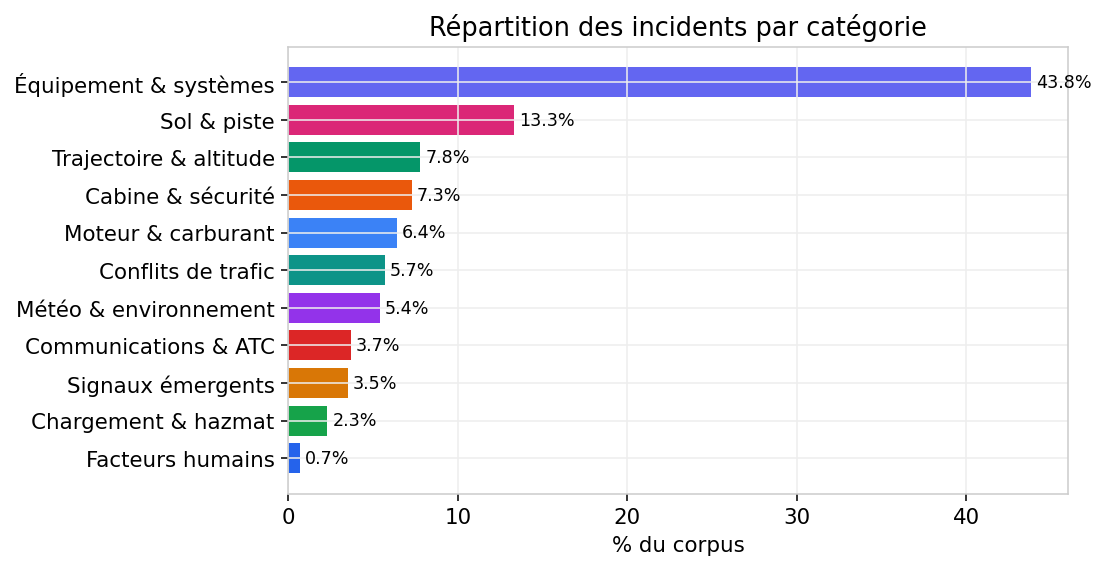
\includegraphics[width=0.80\textwidth]{categories.png}
  \caption{Répartition des incidents par catégorie (regroupement des 81 thèmes en 11 familles).}\label{fig:cat}
\end{figure}

Cette prédominance ne signifie pas que les avions tombent sans cesse en panne : elle traduit
surtout que les équipages \textbf{signalent massivement} le moindre problème technique. Pour
un exploitant, c'est un argument fort en faveur d'une \textbf{maintenance proactive} : la
matière existe pour anticiper les défaillances plutôt que de les subir.

\begin{figure}[h]\centering
  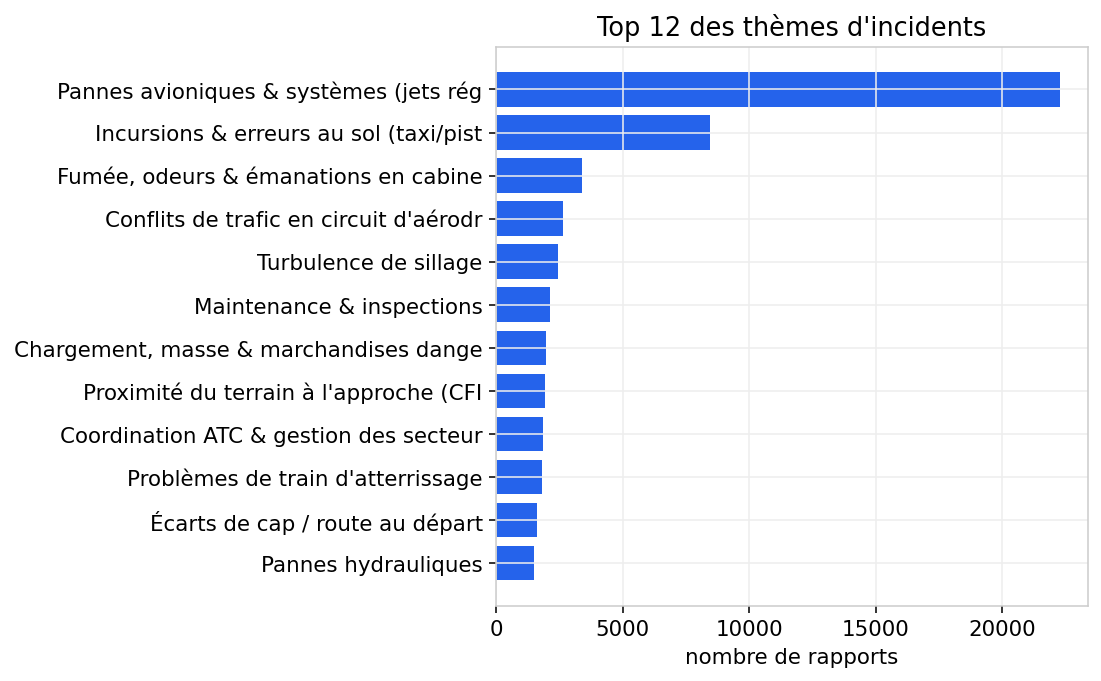
\includegraphics[width=0.80\textwidth]{top_themes.png}
  \caption{Les douze thèmes d'incidents les plus volumineux.}\label{fig:top}
\end{figure}

Chaque thème reçoit un nom métier et des mots-clés caractéristiques (figure~\ref{fig:wc}),
ce qui rend la cartographie immédiatement lisible.

\begin{figure}[h]\centering
  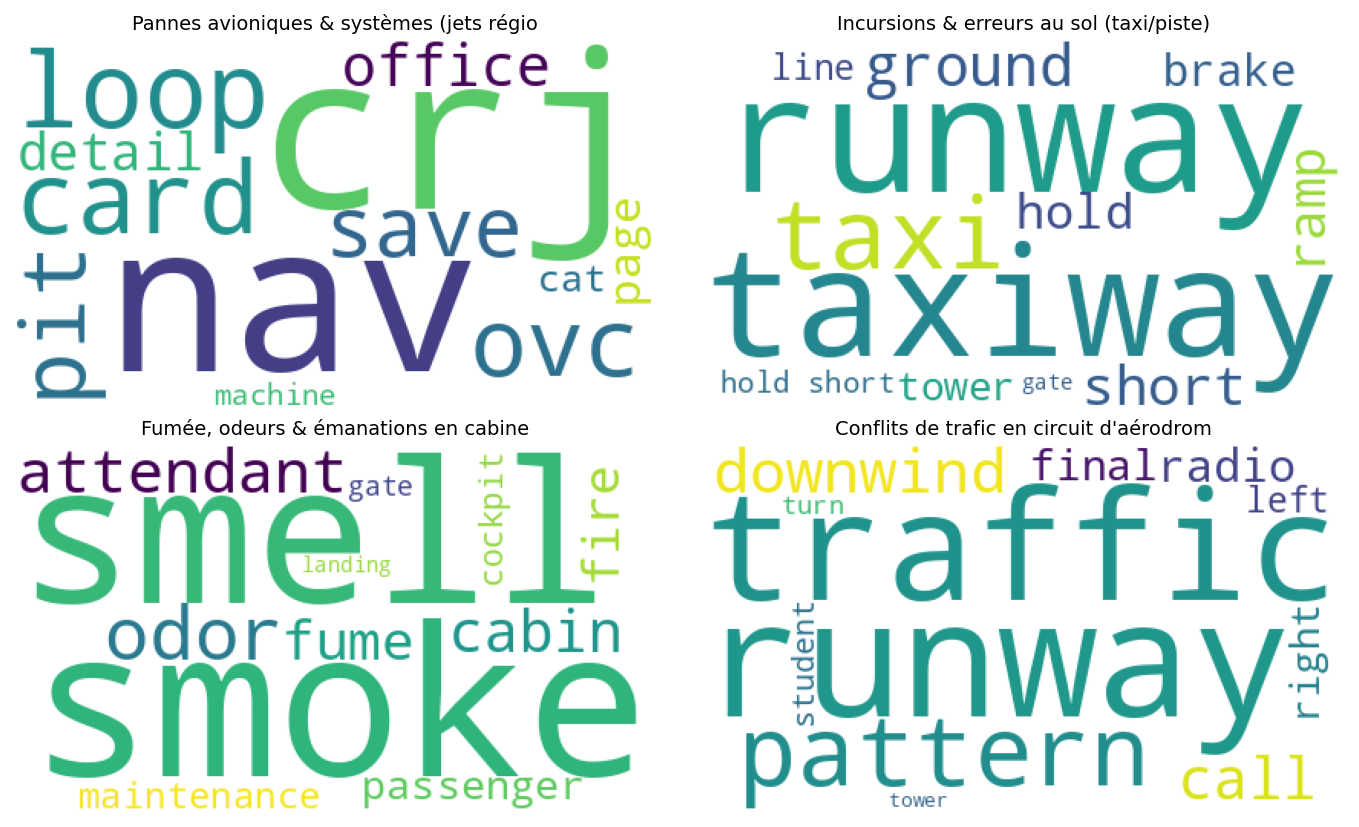
\includegraphics[width=0.92\textwidth]{wordclouds.png}
  \caption{Nuages de mots (c-TF-IDF) des quatre principaux thèmes.}\label{fig:wc}
\end{figure}

\subsection{Quel algorithme de regroupement retenir ?}
Pour comparer K-Means et HDBSCAN, on utilise trois mesures de qualité d'un regroupement :
\begin{itemize}[leftmargin=1.4em,nosep]
  \item le \textbf{score de silhouette (Silhouette Score)}, compris entre $-1$ et $1$ : plus
  il est proche de 1, mieux les points sont regroupés ;
  \item l'\textbf{indice de Davies-Bouldin (Davies-Bouldin Index)} : plus il est \emph{faible},
  mieux les groupes sont séparés ;
  \item le \textbf{score de Calinski-Harabasz (Calinski-Harabasz Score)} : rapport entre la
  dispersion entre groupes et à l'intérieur des groupes ; plus il est élevé, mieux c'est.
\end{itemize}

\begin{table}[h]\centering\small
\caption{Comparaison des deux algorithmes de regroupement.}\label{tab:clust}
\begin{tabular}{lrrrrr}
\toprule
\textbf{Modèle} & \textbf{Clusters} & \textbf{Silhouette} & \textbf{Davies-Bouldin} & \textbf{Bruit} & \textbf{Pureté} \\
\midrule
K-Means & 15 & 0,382 & 0,945 & 0\,\% & 0,133 \\
\textbf{HDBSCAN (retenu)} & \textbf{81} & \textbf{0,590} & \textbf{0,575} & 32\,\% & 0,165 \\
\bottomrule
\end{tabular}
\end{table}
\textbf{HDBSCAN est retenu} : sa silhouette est plus élevée (0,590 contre 0,382) et son
indice de Davies-Bouldin plus faible, signe de groupes mieux séparés. La faible
correspondance avec les catégories officielles d'anomalies (mesurée par la « pureté ») est
normale : les thèmes obtenus sont plus fins que la dizaine de catégories codées par les
analystes. Les 32\,\% de points classés « bruit » ne sont pas jetés : ils alimentent la
détection de signaux faibles.

\subsection{Vérifier que le modèle « comprend » le domaine}
Le modèle Word2Vec apprend, sans aide, des associations pertinentes (tableau~\ref{tab:w2v}) :
par exemple \texttt{runway} (piste) est proche de \texttt{rwy} (son abréviation) et de
\texttt{taxiway} (voie de circulation). Cela confirme la qualité des données. De son côté, la
qualité des sujets LDA se mesure par la \textbf{cohérence $c_v$} (un score indiquant si les
mots d'un sujet vont bien ensemble) : elle atteint 0,57, ce qui correspond à des sujets
lexicalement homogènes.

\begin{table}[h]\centering\small
\caption{Word2Vec — mots les plus proches (similarité cosinus) appris sur le corpus.}\label{tab:w2v}
\begin{tabular}{ll}
\toprule
\textbf{Terme} & \textbf{Voisins les plus proches} \\
\midrule
\texttt{runway}   & rwy (0,84), taxiway (0,65), intersecting (0,59), midfield (0,59) \\
\texttt{engine}   & eng (0,69), feathered (0,57), magneto (0,54), crossbleed (0,54) \\
\texttt{weather}  & thunderstorm (0,76), storm (0,74), bkn (0,68), forecast (0,66) \\
\texttt{altitude} & alt (0,70), descended (0,67), descend (0,65), level (0,64) \\
\bottomrule
\end{tabular}
\end{table}

\subsection{Prédire le type d'incident}
Le score utilisé est le \textbf{F1} : une note entre 0 et 1 qui combine la précision et le
rappel (1 = parfait). On distingue le \emph{F1 macro} (moyenne simple sur toutes les
catégories) et le \emph{F1 pondéré} (qui tient compte de la taille des catégories).

\begin{table}[h]\centering\small
\caption{Performance de la classification (8 catégories d'anomalies, TF-IDF).}\label{tab:clf}
\begin{tabular}{lrr}
\toprule
\textbf{Modèle} & \textbf{F1 macro} & \textbf{F1 pondéré} \\
\midrule
Régression logistique & 0,518 & 0,606 \\
SVM linéaire & 0,517 & \textbf{0,615} \\
\bottomrule
\end{tabular}
\end{table}
Avec un F1 pondéré de 0,615 sur 8 catégories et du texte entièrement libre, le résultat est
satisfaisant. Les catégories au vocabulaire net sont les mieux reconnues (\emph{ATC Issue},
F1\,=\,0,76 ; \emph{NMAC}, 0,69), tandis que les catégories rares restent plus difficiles.

% ---------- 5 ----------
\section{Discussion : tendances et signaux faibles}

Les résultats précédents donnent une photographie ; l'analyse temporelle, elle, donne le
film. En suivant l'évolution des thèmes dans le temps (figures~\ref{fig:vol}
et~\ref{fig:heat}), plusieurs tendances ressortent, dont l'interprétation a un intérêt
opérationnel direct :
\begin{itemize}[leftmargin=1.4em]
  \item \textbf{Incursions et erreurs au sol — en hausse.} Cette progression est cohérente
  avec la \textbf{densification du trafic} : plus d'avions au sol, plus de croisements, donc
  plus d'occasions d'erreur sur les voies de circulation.
  \item \textbf{Fumées et odeurs en cabine — en hausse.} Sujet sensible, qui appelle une
  vigilance accrue sur la qualité de l'air et les circuits de prélèvement.
  \item \textbf{Marchandises dangereuses — en hausse.} Cohérent avec la croissance du fret,
  avec des enjeux de conformité documentaire et de sûreté.
\end{itemize}

\begin{figure}[h]\centering
  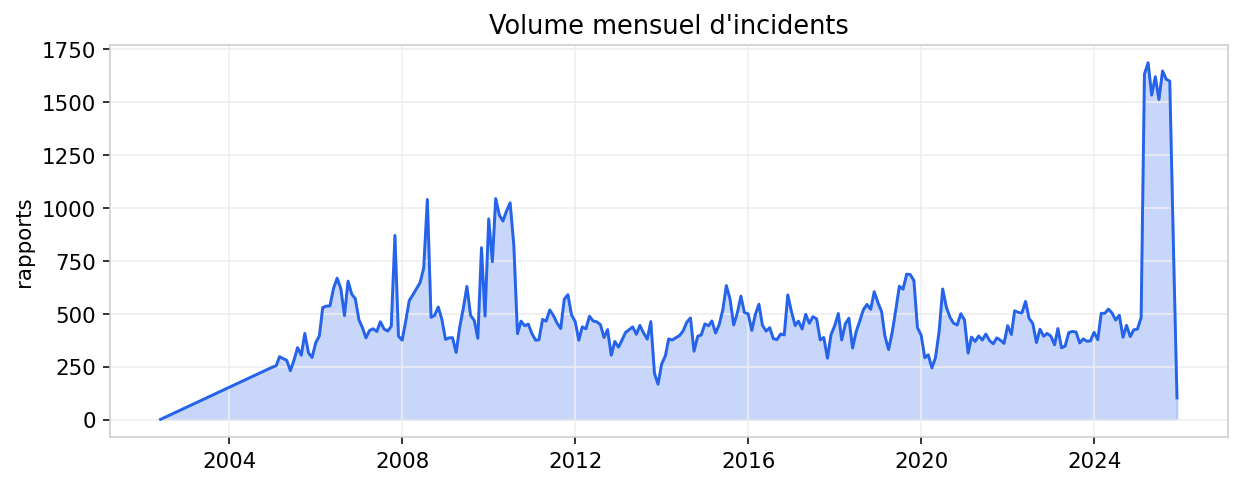
\includegraphics[width=0.84\textwidth]{temporal_volume.png}
  \caption{Volume mensuel de rapports (2002–2025).}\label{fig:vol}
\end{figure}
\begin{figure}[h]\centering
  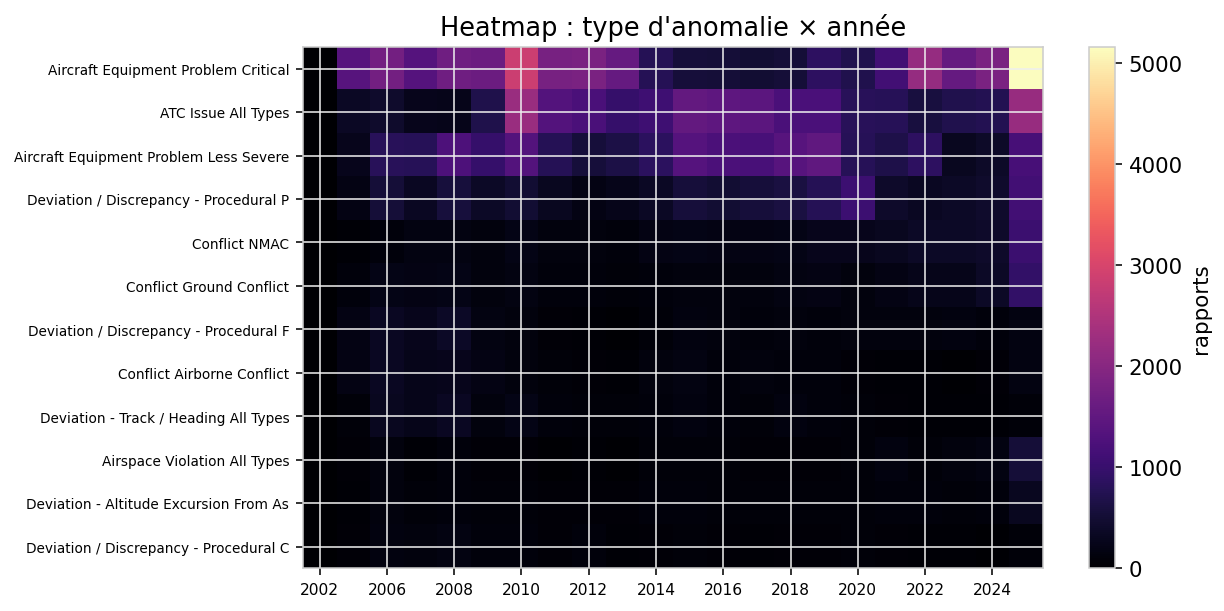
\includegraphics[width=0.84\textwidth]{heatmap.png}
  \caption{Heatmap (carte de chaleur) : type d'anomalie × année.}\label{fig:heat}
\end{figure}

L'apport le plus important concerne les \textbf{signaux faibles}. La détection d'anomalies
fait remonter des phénomènes rares mais lourds de sens : les rencontres avec des
\textbf{drones}, le \textbf{brouillage du signal GPS} et les \textbf{batteries au lithium} —
des sujets quasi inexistants il y a quinze ans. Un récit l'illustre :

\begin{narr}
Approach control advised there was unauthorized drone use in the area\ldots I observed a
drone pass just left of the aircraft, approximately 20 feet from our left wing.
\end{narr}

\noindent Un analyste humain, face à 125\,000 rapports, passerait à côté. Le système, lui, le
fait remonter en tête de liste. C'est précisément la valeur d'un détecteur de signaux
faibles : voir tôt ce qui pourrait devenir, demain, une nouvelle catégorie d'accidents.

% ---------- 6 ----------
\section{Limites et perspectives}

Plusieurs limites encadrent l'interprétation des résultats :
\begin{itemize}[leftmargin=1.4em]
  \item \textbf{Déséquilibre des classes} : certaines catégories sont bien plus fréquentes
  que d'autres, ce qui pénalise la reconnaissance des catégories rares.
  \item \textbf{Données anonymisées} : la suppression des lieux et identifiants fait perdre un
  contexte parfois utile.
  \item \textbf{Biais de déclaration} : l'ASRS étant volontaire, le corpus reflète les
  incidents \emph{signalés}, et non l'ensemble des incidents survenus.
\end{itemize}

\noindent Plusieurs pistes permettraient d'aller plus loin. \textbf{BERTopic} — une méthode
récente de découverte de thèmes combinant embeddings et regroupement, avec suivi temporel
intégré — offrirait une thématisation de bout en bout. Des \textbf{embeddings spécialisés},
ré-entraînés sur un corpus aéronautique, sépareraient mieux les thèmes techniques. Une
\textbf{classification multi-étiquettes} (plusieurs anomalies par rapport) refléterait mieux
la réalité. Enfin, croiser les signaux faibles avec des données externes (trafic, météo)
ouvrirait la voie à une analyse prédictive.

% ---------- 7 ----------
\section{Conclusion}

Le projet part d'une matière brute — 125\,763 récits illisibles à l'échelle humaine — et la
transforme en information structurée : 81 thèmes interprétables regroupés en 11 familles, un
modèle de classification opérationnel (F1 pondéré de 0,615), un dispositif de détection de
signaux faibles, et deux tableaux de bord interactifs accessibles même à un public non
spécialiste.

Au-delà des chiffres, la valeur du travail tient à cette \textbf{transformation de récits
bruts en intelligence exploitable}. En rendant visibles les causes récurrentes, les
tendances et les risques émergents, l'approche fournit un véritable outil d'aide à la
décision pour la sécurité aérienne — et montre, plus largement, comment le traitement
automatique du langage peut valoriser les grandes bases de retour d'expérience.

\vfill
\noindent\footnotesize\textit{Sources des données : NASA Aviation Safety Reporting System
(\url{https://asrs.arc.nasa.gov/}) et jeu équivalent sur Kaggle. Code, dashboards et
reproductibilité : \url{https://github.com/devMehdi485/asrs-ml}.}

\end{document}
